\section{YCbCr}

YCbCr et Y’CbCr sont deux choses différentes. Pour ce projet, YCbCr est utilisé.

YCbCr est une manière de représenter l’espace colorimétrique en vidéo. YCbCr n’est pas un espace de couleur absolu, il est une version compressée et biaisée de YUV (Y : la luminance, U et V : la chrominance). Y représente la luminance, qui représente la densité de la lumière. Cb et Cr sont les deux informations de chrominance. Cb est (Y - bleu), Cr est (Y - rouge).

\begin{figure}[h!]
      \centering
      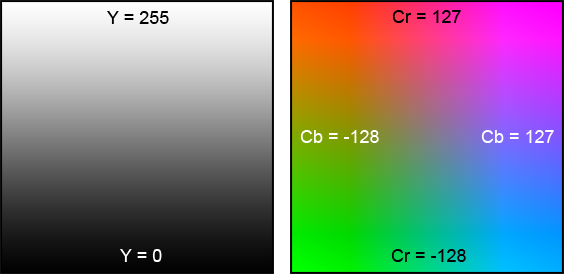
\includegraphics[scale=0.6]{images/YCbCr.png}
      \caption{\label{YCbCr}YCbCr}
\end{figure}


\subsection{Utilisation informatique}
YCbCr est utilisé pour les images JPEG. En comparant avec RGB, ce modèle permet de réduire la taille d’une image. Bien clairement, il peut aussi augmenter l’efficacité de la détection de rupture.

Pour faire la conversion RGB -> YCbCr il faut utiliser les formules suivantes :

\[
 \left \{
 \begin{array}{c @{=} l}
	Y & 0.299 \times R + 0.587 \times G + 0.114 \times B \\
	Cb & -0.1687 \times R - 0.3313 \times G + 0.5 \times B + 128 \\
	Cr & 0.5 \times R - 0.4187 \times G - 0.0813 \times B + 128 \\
 \end{array}
 \right.
\]

Pour faire la conversion YCbCr -> RGB il faut utiliser les formules suivantes :

\[
 \left \{
 \begin{array}{c @{=} l}
	R & Y + 1.402 \times (Cr - 128) \\
	G & Y - 0.34414 \times (Cb - 128) - 0.71414 \times (Cr - 128) \\
	B & Y + 1.772 \times (Cb - 128) \\
 \end{array}
 \right.
\]


\subsection{Point fort}
YCbCr est une méthode similaire à RGB, mais est une solution plus efficace. À l’aide de YCbCr, nous pouvons aussi augmenter l’efficacité de la détection de rupture.
